% =====================================================================
% metodologia.tex
% Responsabilidad única: describir la metodología común a los análisis
% (cribado con regla prerregistrada, protocolo temporal, diseño L16 de
% Taguchi y su contraste con el factorial completo, métricas, habilidad y
% costo de los errores). Cifras: macros Cri*, Dat*, Reg*, Clf*.
% =====================================================================
\section{Metodología}
\label{sec:metodologia}

\subsection{Cribado de análisis con una regla fijada de antemano}
\label{sec:cribado}

Con la misma base se pueden plantear muchas preguntas, y estudiar a fondo
todas habría diluido el trabajo, así que primeramente se armó un catálogo de
\CriCandidatos{} análisis candidatos (\CriCandidatosReg{} de regresión,
\CriCandidatosClf{} de clasificación, \CriCandidatosAgr{} de agrupamiento y
\CriCandidatosBayes{} bayesianos, estos últimos sin cribar porque no
compiten entre sí), cada uno con su objetivo, su unidad de análisis, su
momento de predicción y un valor de negocio de 1 a 3 asignado antes de ver
resultados. Para cada candidato se construyó una tabla de modelado
(\CriTablasConstruidas{} en total), y las \CriAuditoriasSuperadas{} superaron
la auditoría automática de fugas, que comprueba que ninguna variable tenga un
momento posterior al de la predicción.

Después, cada candidato pasa por la misma prueba rápida, solo con
entrenamiento y \DatBloquesCV{} bloques temporales, una línea base, un modelo
lineal o logístico y un árbol de profundidad \CriProfundidadArbol{}, todo sin
afinar (la prueba completa tomó \CriSegundosPrueba{} segundos). La regla de
selección, escrita en el código antes de mirar resultados y sin ajustes
posteriores, es la siguiente:

\begin{itemize}
    \item \textbf{Tamaño mínimo:} un supervisado necesita al menos
          \CriMinimoFilas{} filas de entrenamiento (y, si es de clasificación,
          \CriMinimoPositivos{} positivos), y un agrupamiento al menos
          \CriMinimoFilasAgrupamiento{} filas.
    \item \textbf{Estabilidad:} la habilidad frente a la línea base debe ser
          positiva en todos los bloques, no solo en promedio.
    \item \textbf{No basta una regla simple:} si un árbol que solo ve la mejor
          variable logra el \CriUmbralReglaSimplePct{}\,\% o más de la
          habilidad, el análisis no necesita un modelo y se descarta del
          estudio a fondo.
    \item \textbf{Tendencia a agruparse:} un agrupamiento necesita un
          estadístico de Hopkins mayor que \CriUmbralHopkins{}.
    \item \textbf{Puntaje:} habilidad media (o silueta) por valor de negocio
          dividido entre 3; en cada tipo gana el elegible de mayor puntaje.
\end{itemize}

\begin{figure}[!htbp]
\centering
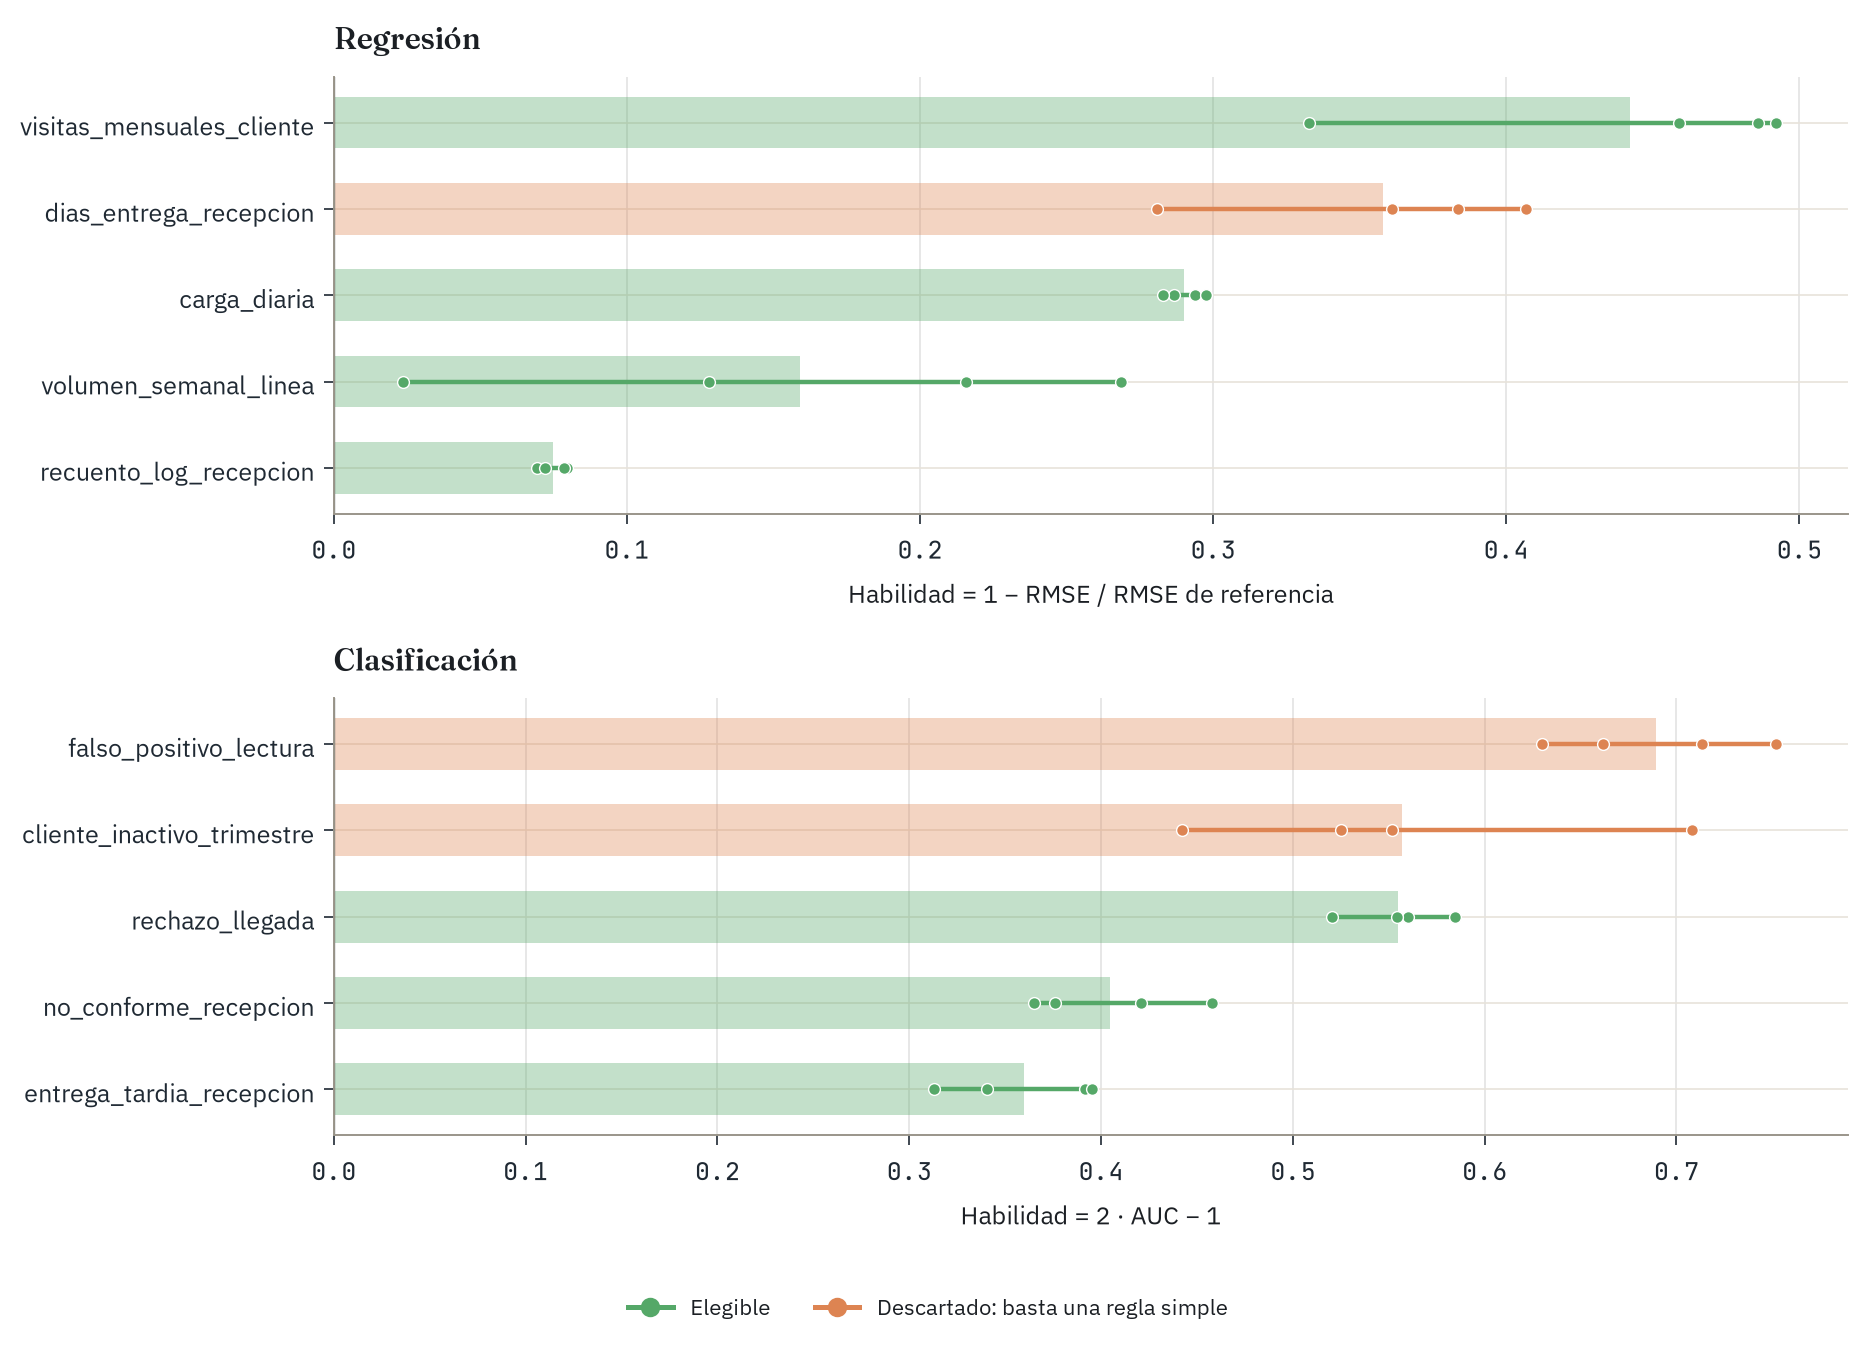
\includegraphics[width=0.66\textwidth]{03_habilidad.png}
\caption{Habilidad de cada supervisado en el cribado (barra: media; puntos:
cada bloque temporal). Los puntos muestran qué tan estable es la habilidad
entre bloques, y el color separa los elegibles de los descartados porque una
sola variable basta.}
\label{fig:cribado}
\end{figure}

De los \CriCribados{} candidatos cribados, \CriElegibles{} resultaron
elegibles, los \CriSupervisadosEstables{} supervisados superaron a su línea
base en todos los bloques y \CriDescartadosReglaSimple{} se descartaron porque
basta una regla simple (Figura~\ref{fig:cribado} y
Tablas~\ref{tab:cribado-reg} y~\ref{tab:cribado-clf}). El caso más ilustrativo
es \codigo{\CriClfMasHabil}, el clasificador con la mayor habilidad bruta
(\CriClfMasHabilHabilidad{}), del que la mejor variable sola logra el
\CriClfMasHabilProporcion{}\,\%, es decir, que en lugar de un modelo basta una
regla sobre el recuento, y esa regla es justamente la que se desarrolla en la
Sección~\ref{sec:bayes}. En regresión ocurre algo parecido con
\codigo{dias\_entrega\_recepcion}, que tiene más habilidad que el elegido pero
la explica casi entera el plazo prometido. El candidato más inestable,
\codigo{\CriMasInestable}, pasa de una habilidad de \CriMasInestableMin{} a
\CriMasInestableMax{} entre bloques.

\begin{table}[!htbp]
\centering
\tablaancha{cribado_regresion}
\caption{Cribado de los análisis de regresión (solo entrenamiento). La
habilidad es $1-\mathrm{RMSE}/\mathrm{RMSE}_\text{base}$ y la proporción de la
regla es la fracción de esa habilidad que logra la mejor variable sola.}
\label{tab:cribado-reg}
\end{table}

\begin{table}[!htbp]
\centering
\tablaancha{cribado_clasificacion}
\caption{Cribado de los análisis de clasificación (solo entrenamiento). La
habilidad es $2\cdot\mathrm{AUC}-1$; una proporción de la regla mayor que 1
indica que la variable sola supera al modelo.}
\label{tab:cribado-clf}
\end{table}

La regla eligió \codigo{\CriSeleccionReg} en regresión (habilidad
\CriSeleccionRegHabilidad{}, puntaje \CriSeleccionRegPuntaje{}),
\codigo{\CriSeleccionClf} en clasificación (ROC-AUC
\CriSeleccionClfAUC{}, puntaje \CriSeleccionClfPuntaje{}) y
\codigo{\CriSeleccionAgr} en agrupamiento (silueta
\CriSeleccionAgrSilueta{} con $k=\CriMejorSiluetaK$, Hopkins entre
\CriHopkinsMin{} y \CriHopkinsMax{} entre los candidatos). El agrupamiento
\codigo{\CriAgrComplementario} se estudia también, pero como análisis
complementario, fuera de la regla.

\subsection{Protocolo temporal}
\label{sec:protocolo}

Como los datos son una serie en el tiempo, la partición no es aleatoria sino
por fecha de recepción (Figura~\ref{fig:protocolo} y
Tabla~\ref{tab:particion}), de forma que todo modelo se evalúa siempre sobre
un periodo posterior al que vio. Dentro de entrenamiento, la validación
cruzada usa bloques de ventana creciente, y la partición de prueba solo puede
leerse a través de una función que existe en la etapa~07, la cual registra
cada lectura en un archivo que la verificación automática revisa.

% =====================================================================
% protocolo.tex
% Responsabilidad única: dibujar el protocolo temporal del proyecto
% (entrenamiento, validación y prueba por fechas; qué se hace con cada bloque;
% validación cruzada de ventana creciente y punto de congelamiento). Fechas y
% tamaños son macros generadas por los notebooks.
% =====================================================================
\begin{figure}[!htbp]
\centering
\begin{tikzpicture}[
    every node/.style={font=\small},
    caja/.style={draw, rounded corners=2pt, align=center, minimum height=1.05cm, inner sep=4pt},
    paso/.style={draw, rounded corners=2pt, align=center, fill=gray!6, text width=4.2cm,
                 minimum height=1.9cm, inner sep=4pt},
    flecha/.style={-{Stealth[length=2.2mm]}, thick},
]
% --- Datos y partición por fechas ------------------------------------------
\node[caja, fill=gray!10, text width=15.2cm] (datos) at (0,0)
    {\textbf{Datos:}\enspace \ExpMuestrasLimpias{} muestras limpias recibidas entre \DatDesde{} y \DatHasta{}\\[1pt]
     {\scriptsize\color{gray!70!black}partición por fecha de recepción, sin mezclar: Cortes en \DatCorteValidacion{} y \DatCortePrueba{}}};

\node[caja, fill=classblue!14, draw=classblue, text width=4.2cm] (tr) at (-5.3,-2.2)
    {\textbf{Entrenamiento}\\ antes de \DatCorteValidacion{}\\ \ExpFilasEntrenamiento{} muestras, \RegDiasEntrenamiento{} días};
\node[caja, fill=classgreen!16, draw=classgreen, text width=4.2cm] (val) at (0,-2.2)
    {\textbf{Validación}\\ \DatCorteValidacion{} a \DatCortePrueba{}\\ \ExpFilasValidacion{} muestras, \RegDiasValidacion{} días};
\node[caja, fill=classred!12, draw=classred, text width=4.2cm] (te) at (5.3,-2.2)
    {\textbf{Prueba}\\ desde \DatCortePrueba{}\\ \ExpFilasPrueba{} muestras, \FinDiasPrueba{} días};

\foreach \n in {tr, val, te} \draw[flecha, gray] (datos.south -| \n) -- (\n.north);

% --- Qué se hace con cada bloque ------------------------------------------
\node[paso, below=0.75cm of tr] (ajuste)
    {\textbf{Ajustar y explorar}\\ cribado, L16 de Taguchi y rejilla, con validación cruzada temporal};
\node[paso, below=0.75cm of val] (decidir)
    {\textbf{Decidir y congelar}\\ modelo, calibración y umbral por costo; Reajuste con entrenamiento + validación};
\node[paso, below=0.75cm of te] (evaluar)
    {\textbf{Evaluar una sola vez}\\ Etapa 07: Métricas con intervalos bootstrap, sin cambiar nada};

\draw[flecha, classblue] (tr) -- (ajuste);
\draw[flecha, classgreen] (val) -- (decidir);
\draw[flecha, classred] (te) -- (evaluar);
\draw[flecha] (ajuste) -- (decidir);
\draw[flecha] (decidir) -- (evaluar);

% --- Barrera de congelamiento ----------------------------------------------
\coordinate (barrera) at ($(te.west)+(-0.28,0)$);
\draw[classred, very thick, dashed] ($(barrera)+(0,0.9)$) -- ($(barrera |- evaluar.south)+(0,-0.1)$);
\node[classred, font=\scriptsize\bfseries, align=center, fill=white, inner sep=1pt]
    at ($(barrera)+(0,1.2)$) {lectura única y registrada};

% --- Validación cruzada de ventana creciente (dentro de entrenamiento) ------
\begin{scope}[shift={($(ajuste.south)+(-2.1,-0.55)$)}]
  \node[font=\scriptsize, anchor=west, gray!70!black] at (0,0)
      {\DatBloquesCV{} bloques de ventana creciente (solo entrenamiento):};
  \foreach \i/\a in {1/1.6, 2/2.3, 3/3.0, 4/3.7} {
    \fill[classblue!45] (0,-0.28*\i-0.12) rectangle (\a,-0.28*\i+0.04);
    \fill[classgreen!70] (\a,-0.28*\i-0.12) rectangle (\a+0.7,-0.28*\i+0.04);
  }
  \node[font=\scriptsize, anchor=west] at (4.6,-0.55) {\textcolor{classblue}{ajusta}};
  \node[font=\scriptsize, anchor=west] at (4.6,-0.9) {\textcolor{classgreen!70!black}{valida}};
\end{scope}
\end{tikzpicture}
\caption{Protocolo temporal del proyecto, donde cada bloque de fechas cumple
un solo papel: Con entrenamiento ajustamos y exploramos configuraciones con
validación cruzada de ventana creciente (abajo a la izquierda, donde cada
pliegue entrena con el pasado y valida con el tramo siguiente). Con
validación decidimos y congelamos. La prueba se abre una sola vez en la
etapa~07, que deja registrada cada lectura.}
\label{fig:protocolo}
\end{figure}


\begin{table}[!htbp]
\centering
\small
\tablagen{particion}
\caption{Muestras por bloque temporal (todas las muestras limpias, por fecha
de recepción). Cada análisis tiene su propia unidad, por ejemplo días hábiles
en la regresión, pero respeta los mismos cortes.}
\label{tab:particion}
\end{table}

\subsection{Diseño ortogonal L16 de Taguchi}
\label{sec:taguchi}

Para cada análisis elegido quedan seis decisiones de diseño, el modelo
(KNN, lineal o logístico, árbol o perceptrón multicapa, a cuatro niveles), el
escalado (estándar o min-max), el grupo de variables (base o ampliado), la
selección de variables por $F$ (ninguna o las $k$ mejores), la codificación
de categóricas (one-hot u ordinal) y un sexto factor propio de cada tarea
(objetivo en logaritmo en la regresión, sobremuestreo de la clase minoritaria
en la clasificación). El factorial completo tiene
$4\times 2^5=\RegCorridasCompleto$ combinaciones, y en lugar de correrlas
todas se usa un arreglo ortogonal L16, que con 16 corridas mantiene cada par
de factores balanceado.

\paragraph{Estructura de alias.} El factor de cuatro niveles ocupa tres
columnas del arreglo (dos columnas base y su interacción), el escalado otra,
y los cuatro factores restantes columnas generadas por productos, de forma
que tres columnas (\codigo{ac}, \codigo{bc} y \codigo{abc}) quedan libres para
estimar la interacción modelo $\times$ escalado, la que más se esperaba (KNN y
el perceptrón dependen de la escala, el árbol no). De las
\RegInteracciones{} interacciones de dos factores, \RegInteraccionesLibres{}
quedan libres de confusión con un efecto principal; las demás comparten
columna con otro efecto y por eso el método supone, y luego comprueba con una
corrida de confirmación, que no son grandes.

\paragraph{Razón señal/ruido.} Cada corrida se evalúa en los
\DatBloquesCV{} bloques temporales, y sus puntajes $y_1,\dots,y_n$ se
resumen en una razón señal/ruido (S/N, en dB) que premia a la vez el buen
promedio y la poca variación entre bloques:
\[
\text{S/N}_\text{menor} = -10\log_{10}\Bigl(\tfrac{1}{n}\textstyle\sum_i y_i^2\Bigr)
\quad\text{(RMSE)},\qquad
\text{S/N}_\text{mayor} = -10\log_{10}\Bigl(\tfrac{1}{n}\textstyle\sum_i y_i^{-2}\Bigr)
\quad\text{(ROC-AUC)}.
\]
Con las 16 corridas se construye la tabla de respuesta (S/N medio de cada
nivel, delta entre el mejor y el peor nivel y rango de cada factor), y el
modelo aditivo predice la S/N de la combinación de mejores niveles. Esa
combinación se corre de verdad (corrida de confirmación) y, si la S/N
observada cae dentro de una tolerancia de la predicha, se acepta que las
interacciones no rompen el modelo aditivo. Finalmente, la mejor configuración
(confirmación o mejor corrida observada) pasa a una búsqueda en rejilla de
sus hiperparámetros con los mismos bloques temporales.

\paragraph{Contraste con el factorial completo.} En la regresión, donde cada
corrida es barata, se corrió además el factorial completo
(\RegCorridasCompleto{} corridas, \RegSegundosCompleto{} segundos frente a
\RegSegundosLSixteen{} del L16) para comprobar si el atajo cambia las
conclusiones. La correlación de Spearman entre los deltas de ambos diseños es
de \RegRhoCompleto{}, \RegFactoresMismoOptimo{} de los \RegFactores{} factores
tienen el mismo mejor nivel en ambos, y el orden de los dos factores más
influyentes, modelo y grupo, se conserva (Figura~\ref{fig:l16-completo}). La
mejor S/N del factorial completo (\RegSNMejorCompleto{} dB) es apenas mayor
que la mejor corrida del L16 (\RegSNMejorCorrida{} dB), y la confirmación
quedó en el puesto \RegPuestoConfirmacion{} de las \RegCorridasCompleto{}
combinaciones. En la clasificación el factorial completo no se corrió (se
estimaron \ClfSegundosCompletoEstimados{} segundos, frente a
\ClfSegundosLSixteen{} del L16), y por eso allí la corrida de confirmación es
la única comprobación del modelo aditivo.

\begin{figure}[!htbp]
\centering
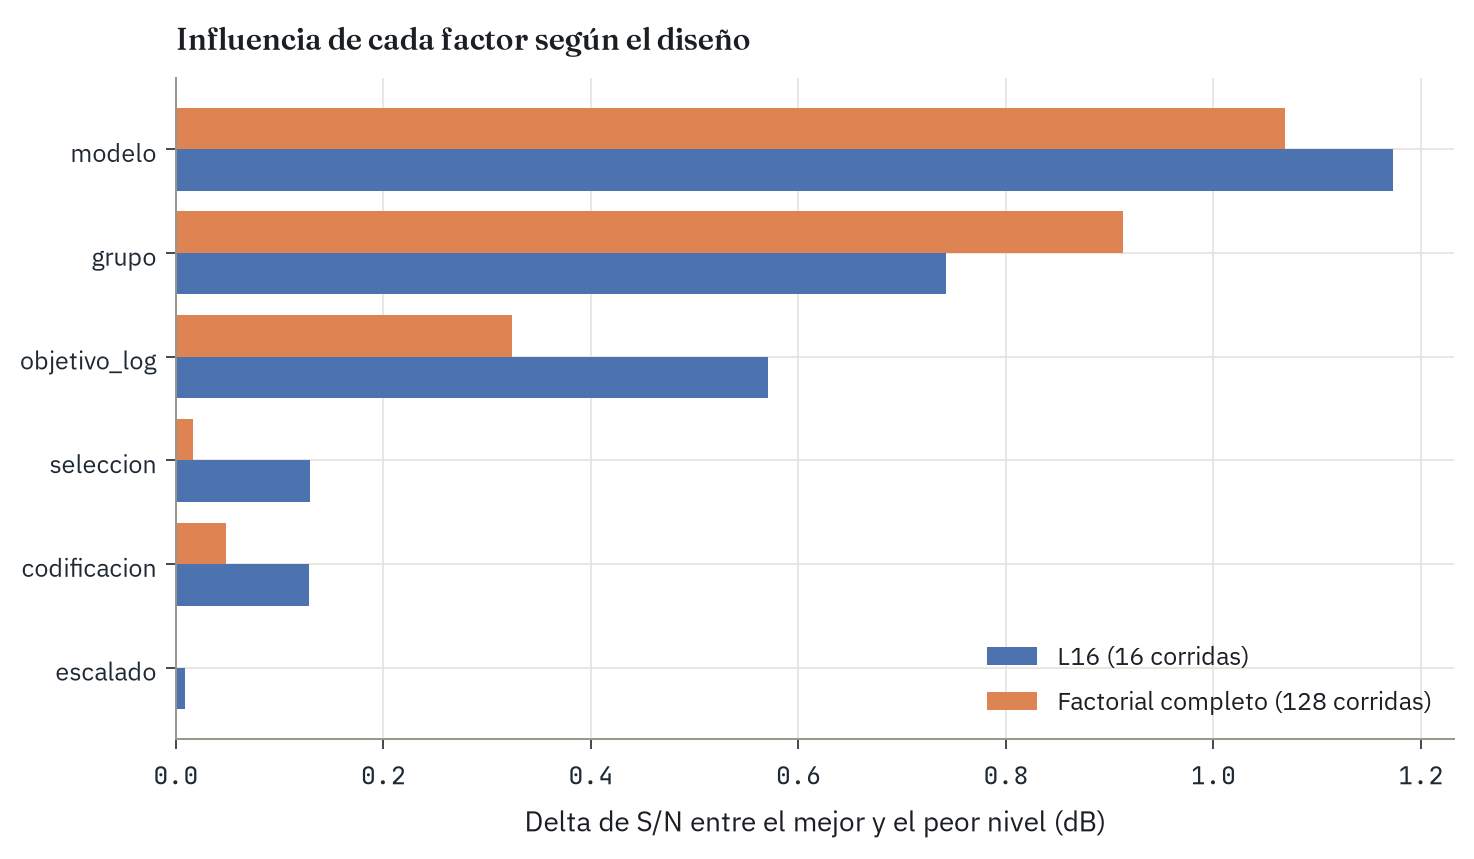
\includegraphics[width=0.5\textwidth]{04_l16_contra_completo.png}
\caption{Delta de S/N de cada factor de la regresión según el L16 (azul) y
el factorial completo (naranja). Lo que importa es que el orden de los
factores y la separación entre los influyentes (modelo, grupo, objetivo en
logaritmo) y los despreciables (escalado) se mantiene con una octava parte de
las corridas.}
\label{fig:l16-completo}
\end{figure}

\subsection{Métricas, habilidad y costo de los errores}
\label{sec:metricas}

Las métricas siguen los temas del curso \cite{muller2016,hastie2009}, con dos
añadidos para que las cifras se puedan comparar entre análisis:

\begin{itemize}
    \item \textbf{Regresión:} MAE, RMSE y $R^2$. La \emph{habilidad} es
          $1-\mathrm{RMSE}/\mathrm{RMSE}_\text{ref}$, donde la referencia es la
          mejor regla ingenua, por ejemplo la media de los cinco días
          hábiles anteriores (\codigo{base\_media\_5}); una habilidad de cero
          significa no mejorar lo que ya se haría sin modelo.
    \item \textbf{Clasificación:} ROC-AUC, precisión media (área bajo la curva
          de precisión y recall, más exigente con el desbalance) y puntaje de
          Brier (error cuadrático de la probabilidad, que mide calibración). La
          habilidad es $2\cdot\mathrm{AUC}-1$, que vale cero para un
          clasificador al azar.
    \item \textbf{Incertidumbre:} las métricas de validación y prueba llevan
          intervalos bootstrap de 95\,\%, y las proporciones (por ejemplo,
          reensayos conformes) intervalos de Wilson.
\end{itemize}

\paragraph{Costo de los errores.} En la clasificación, dejar pasar una muestra
no conforme sin alerta (falso negativo) cuesta \DatCostoFN{} veces lo que
revisar una que resulta conforme (falso positivo, costo \DatCostoFP{}), de
forma que el costo total es
$L=C_\text{FP}\cdot\text{FP}+C_\text{FN}\cdot\text{FN}$. Si las
probabilidades están calibradas, el umbral que minimiza el costo esperado es
$t^\ast=C_\text{FP}/(C_\text{FP}+C_\text{FN})$, que aquí vale
\ClfUmbralTeorico{}; el umbral se elige en validación y se compara con ese
valor teórico. Como un costo bajo puede esconder una avalancha de falsas
alarmas, junto al costo se reportan siempre la precisión y las alertas por
semana.
